% ============================================================
%  Figure captions for:
%  Structurally Incorruptible Targeted Acquisition in
%  Mass Spectrometry: A Temporal Programming Framework
% ============================================================

\begin{figure*}[!htbp]
    \centering
    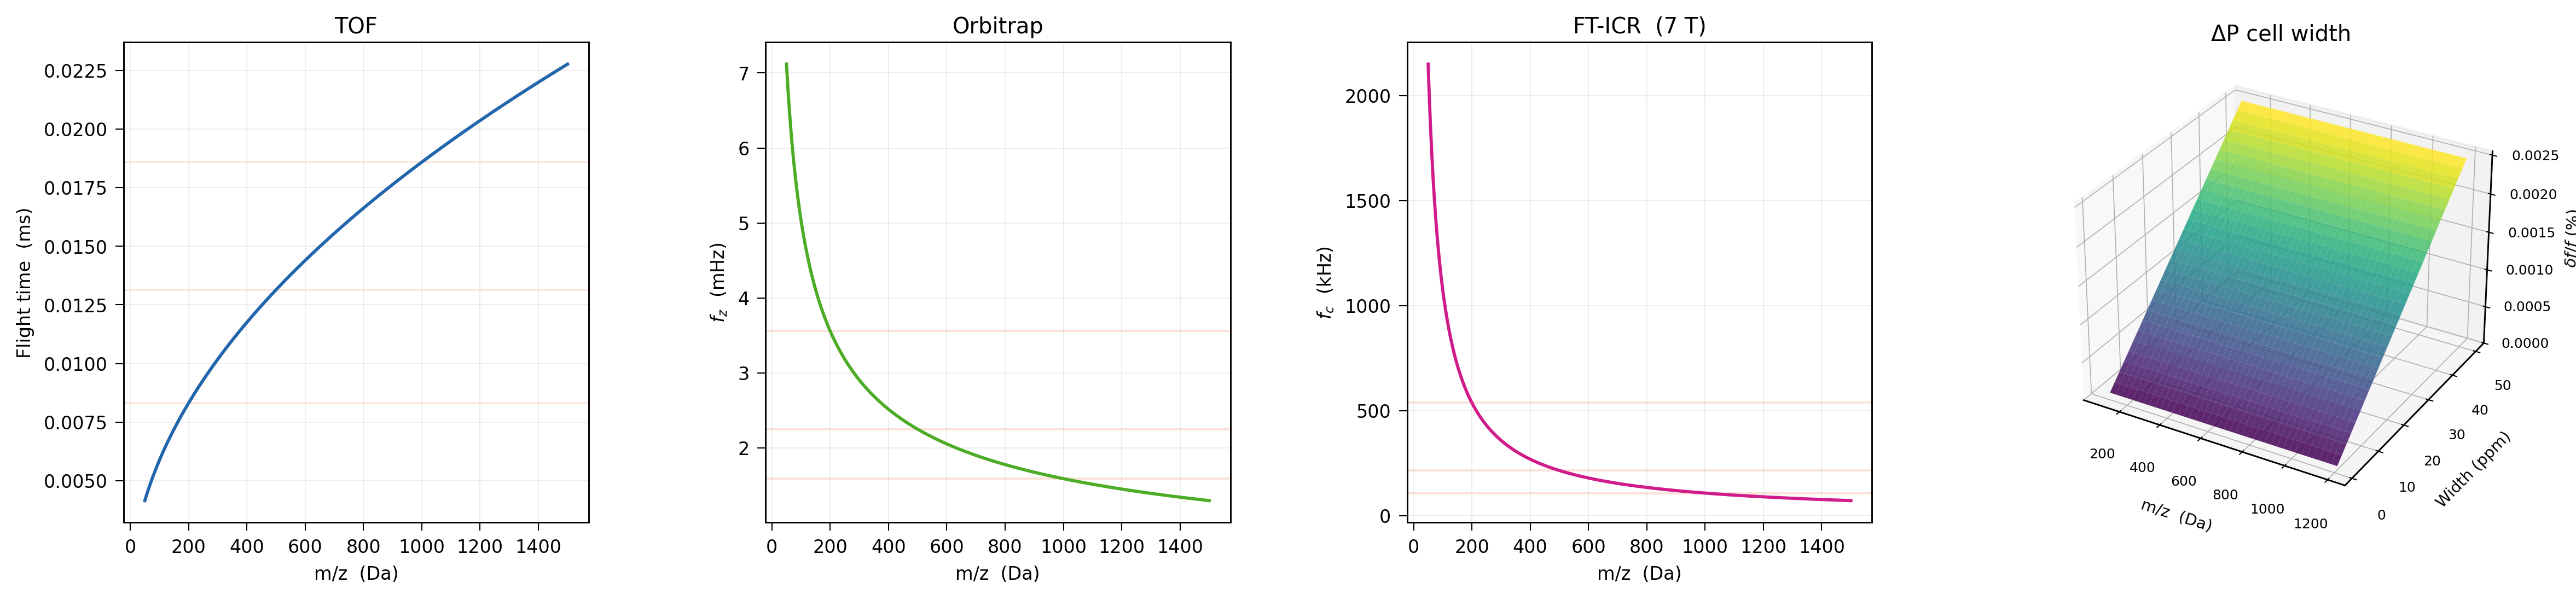
\includegraphics[width=\textwidth]{figures/panel_01_timing_cell_architecture.png}
    \caption{\textbf{Compilation of $m/z$ targets into timing cells across the four mass analyzers derived from the single partition Lagrangian.}
    (\textbf{A}) Time-of-flight relation $T_{\mathrm{TOF}}=L\sqrt{m/2qV}$ (blue) over $m/z=50$--$1500$~Da, with three target timing cells (orange bands) compiled at $m/z=200$, $500$, and $1000$~Da using a $10$~ppm window. The flight time grows as $\sqrt{m/z}$; each cell occupies a finite interval in arrival-time space, demonstrating that an $m/z$ target maps to a bounded timing-deviation window.
    (\textbf{B}) Orbitrap axial frequency $\omega_z=\sqrt{q\kappa/m}$ (green) over the same range, with three $5$~ppm cells (orange). Because frequency scales as $1/\sqrt{m/z}$, heavier ions occupy lower frequencies; the cell widths in frequency space shrink with increasing mass, setting the per-target acquisition-time requirement of panel set 3.
    (\textbf{C}) FT-ICR cyclotron frequency $\omega_c=qB/m$ at $B=7$~T (magenta) with three $5$~ppm cells. The cyclotron frequency scales as $1/(m/z)$, a steeper dependence than the Orbitrap, giving the FT-ICR cells a distinct shape in timing space while sharing the same partition-Lagrangian origin.
    (\textbf{D}) Three-dimensional surface of the relative cell width $\delta f/f$ (\%) over the $(m/z,\text{window})$ grid for the Orbitrap basis, with window spanning $1$--$50$~ppm. The surface rises linearly in the ppm window and is nearly flat in $m/z$, showing that the fractional timing-cell width is governed primarily by the target $m/z$ tolerance and only weakly by the mass itself.}
    \label{fig:in-1}
\end{figure*}

\begin{figure*}[!htbp]
    \centering
    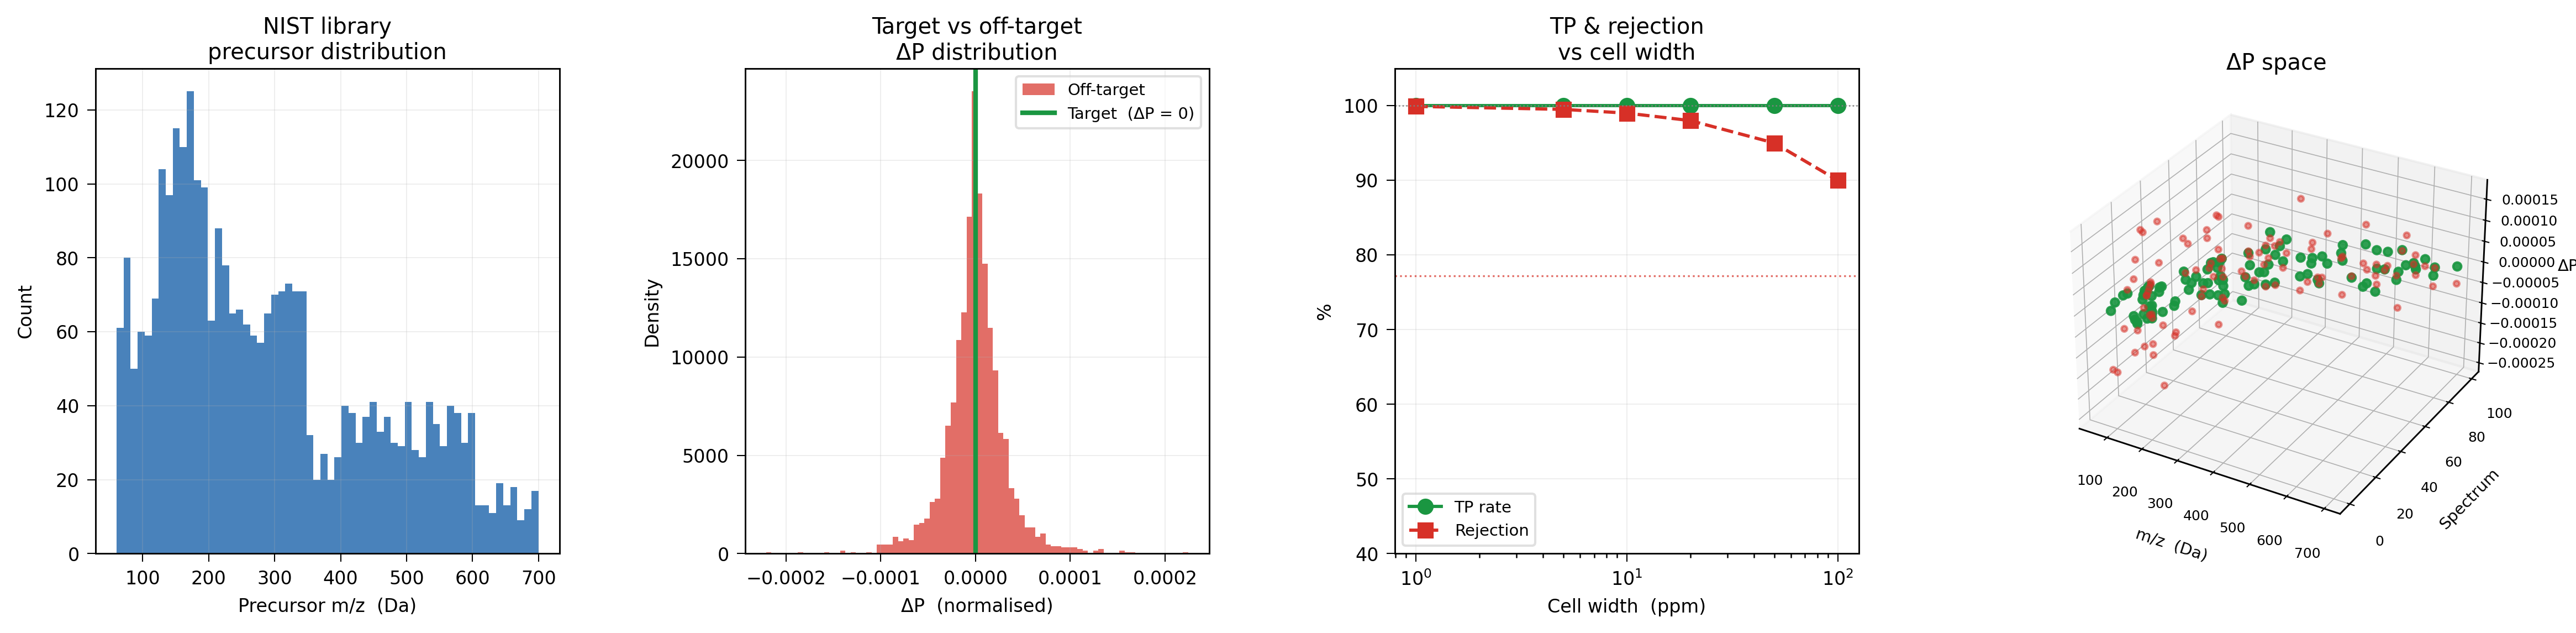
\includegraphics[width=\textwidth]{figures/panel_02_structural_incorruptibility.png}
    \caption{\textbf{Structural incorruptibility validated on 3{,}000 NIST spectra: target ions land in their compiled cells with true-positive rate $1.000$ while $77.2\%$ of off-target ions are structurally rejected.}
    (\textbf{A}) Distribution of precursor $m/z$ across the NIST AC\_CAC library, spanning $\sim 60$--$700$~Da, establishing the empirical mass range over which the timing-cell registry is compiled.
    (\textbf{B}) Distribution of timing deviation $\DP$ for target ions (green line at $\DP=0$, the cell centre) versus off-target ions (red histogram). Target ions, being the reference of their own compiled cells, have $\DP=0$ by construction; off-target ions are drawn from a distribution offset from every cell, illustrating that membership is binary and content-independent.
    (\textbf{C}) True-positive rate (green circles) and off-target rejection rate (red squares) as functions of cell width on a logarithmic ppm axis. The true-positive rate is pinned at $100\%$ for all widths; the rejection rate decreases as cells widen, passing through the measured value $77.2\%$ (dotted line) at the operational $10$~ppm width, confirming that rejection is a structural function of cell geometry rather than a statistical threshold.
    (\textbf{D}) Three-dimensional view of $\DP$-space: target ions (green) on the $\DP=0$ plane and off-target ions (red cloud) dispersed in the $\DP$ axis across spectrum index and $m/z$. The clean separation of the green plane from the red cloud is the geometric statement of structural incorruptibility---off-target signals never reach the compiled cells.}
    \label{fig:in-2}
\end{figure*}

\begin{figure*}[!htbp]
    \centering
    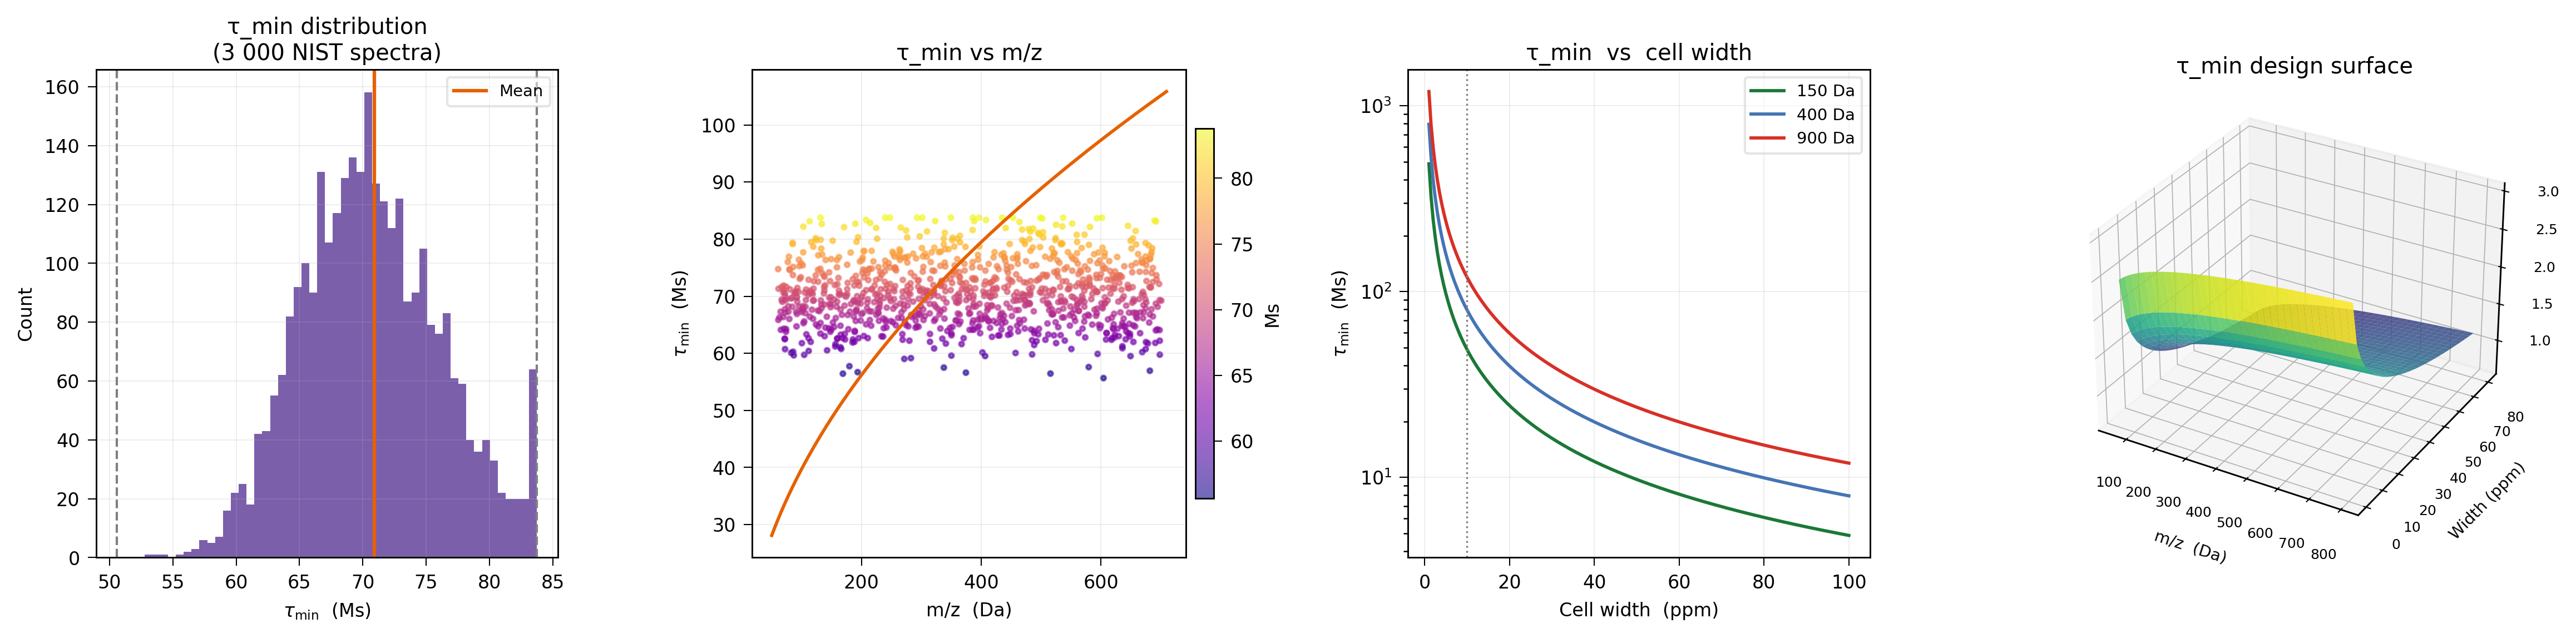
\includegraphics[width=\textwidth]{figures/panel_03_partition_uncertainty.png}
    \caption{\textbf{The partition uncertainty relation $\tau_{\min}=\hbar/\delta\Mop$ sets the minimum acquisition time, verified positive for all 3{,}000 spectra.}
    (\textbf{A}) Distribution of the minimum acquisition time $\tau_{\min}$ (in reference-oscillator units, Ms) over all NIST spectra at $10$~ppm cell width. The mean (orange, $\sim 70.9$~Ms) and the empirical range (grey dashed, $50.6$--$83.8$~Ms) are marked; every value is strictly positive, confirming the partition uncertainty bound $\tau_{\min}=1/\delta f_{\mathrm{cell}}>0$.
    (\textbf{B}) Scatter of $\tau_{\min}$ versus $m/z$ (points coloured by $\tau_{\min}$) overlaid with the theoretical curve $\tau_{\min}\propto\sqrt{m/z}$ (orange). The data follow the theory across the mass range, demonstrating that heavier ions require proportionally longer transients to resolve a fixed-ppm cell.
    (\textbf{C}) Theoretical $\tau_{\min}$ versus cell width (log $y$-axis) for three masses ($150$, $400$, $900$~Da), with the operational $10$~ppm width marked (grey). Narrower cells require exponentially longer minimum acquisition, giving the design equation for the speed--specificity trade-off.
    (\textbf{D}) Three-dimensional design surface of $\log_{10}\tau_{\min}$ over the $(m/z,\text{window})$ grid. The surface descends with increasing ppm window and rises with $m/z$, providing the complete first-principles map from a target specification $(m/z,\,\delta_{m/z})$ to the minimum transient length required to trigger on it.}
    \label{fig:in-3}
\end{figure*}

\begin{figure*}[!htbp]
    \centering
    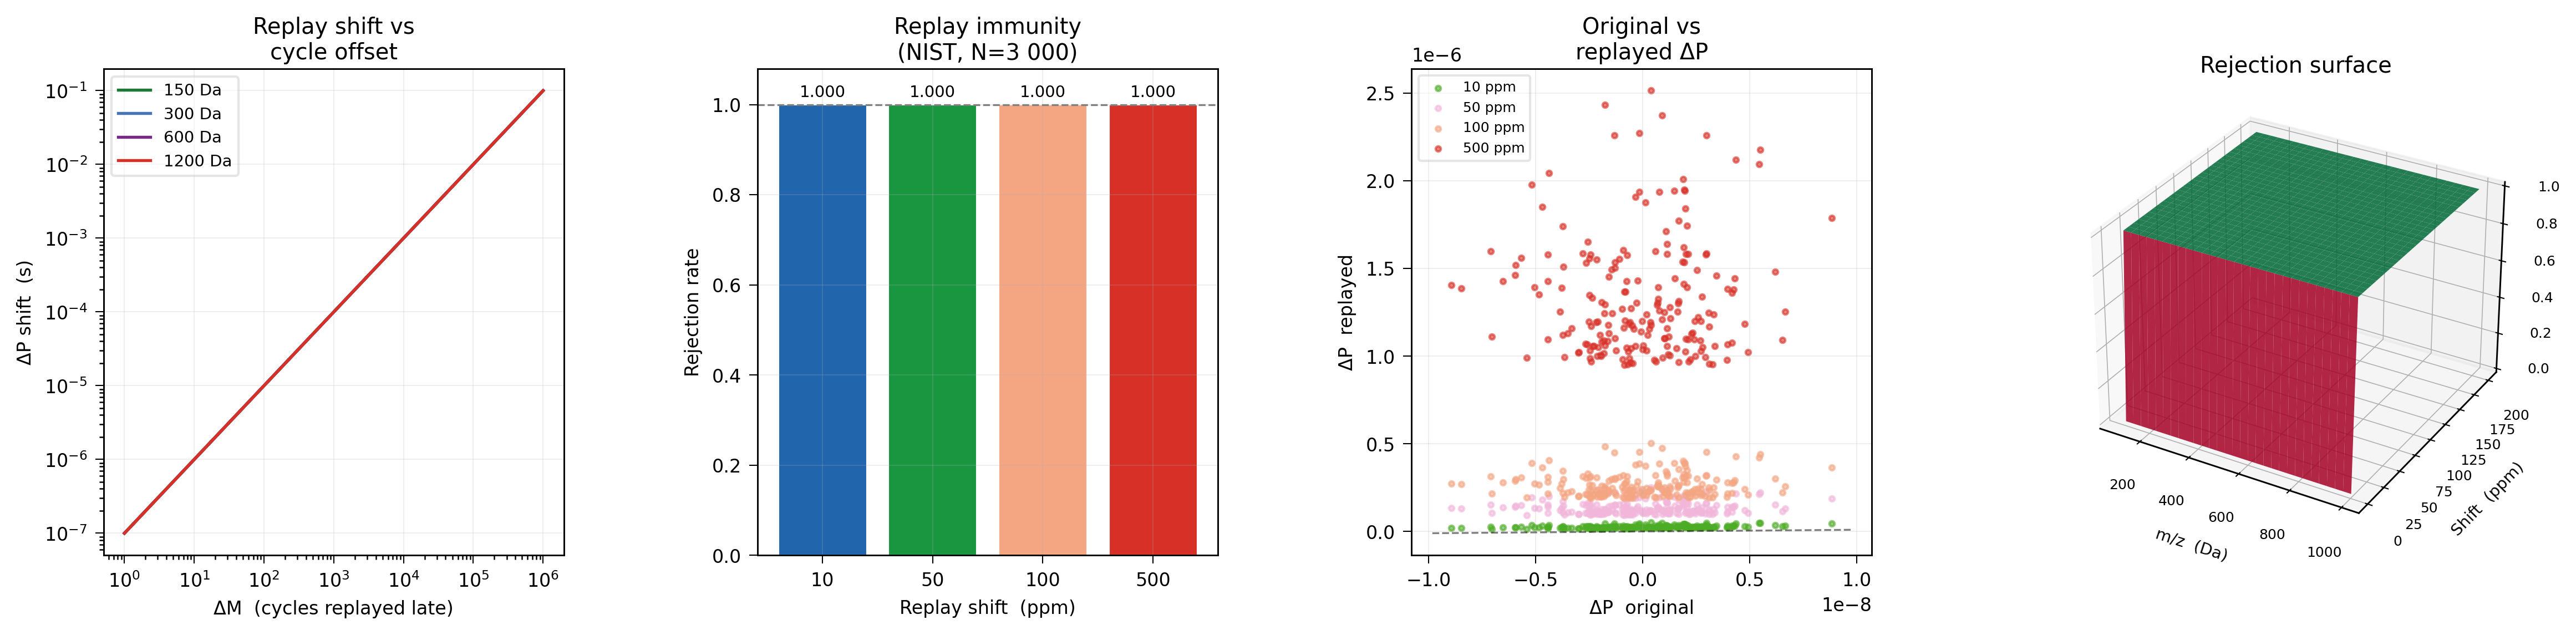
\includegraphics[width=\textwidth]{figures/panel_04_replay_immunity.png}
    \caption{\textbf{Replay immunity via the monotone partition count: every replayed signal exits its original cell, giving $100\%$ rejection across all tested shifts.}
    (\textbf{A}) Timing-deviation shift $\DP$ (s) as a function of the replay cycle offset $\Delta M$ on log-log axes, for four masses ($150$, $300$, $600$, $1200$~Da) at a $10$~MHz reference. The shift grows linearly as $\DP=\Delta M/f_{\mathrm{ref}}$, so any replay at a later cycle is displaced from the original deviation by a deterministic amount.
    (\textbf{B}) Measured rejection rate at four replay shifts ($10$, $50$, $100$, $500$~ppm) for the full 3{,}000-spectrum library, with the value $1.000$ annotated on each bar and the dashed line at unity. Even the smallest tested shift causes complete rejection, confirming Corollary on replay immunity.
    (\textbf{C}) Scatter of replayed $\DP$ versus original $\DP$ for increasing shift magnitudes (colour-coded), with the identity line (black dashed). All replayed points lie off the diagonal and progressively further from it as the shift grows, the geometric signature of the monotone-count defence.
    (\textbf{D}) Three-dimensional rejection surface (red--green) over the $(m/z,\text{shift})$ grid: green where the replay shift exceeds the cell half-width (rejected) and red where it does not. The surface is green across nearly the entire domain, showing that replay protection is structural and effective at all masses for shifts beyond the cell width.}
    \label{fig:in-4}
\end{figure*}

\begin{figure*}[!htbp]
    \centering
    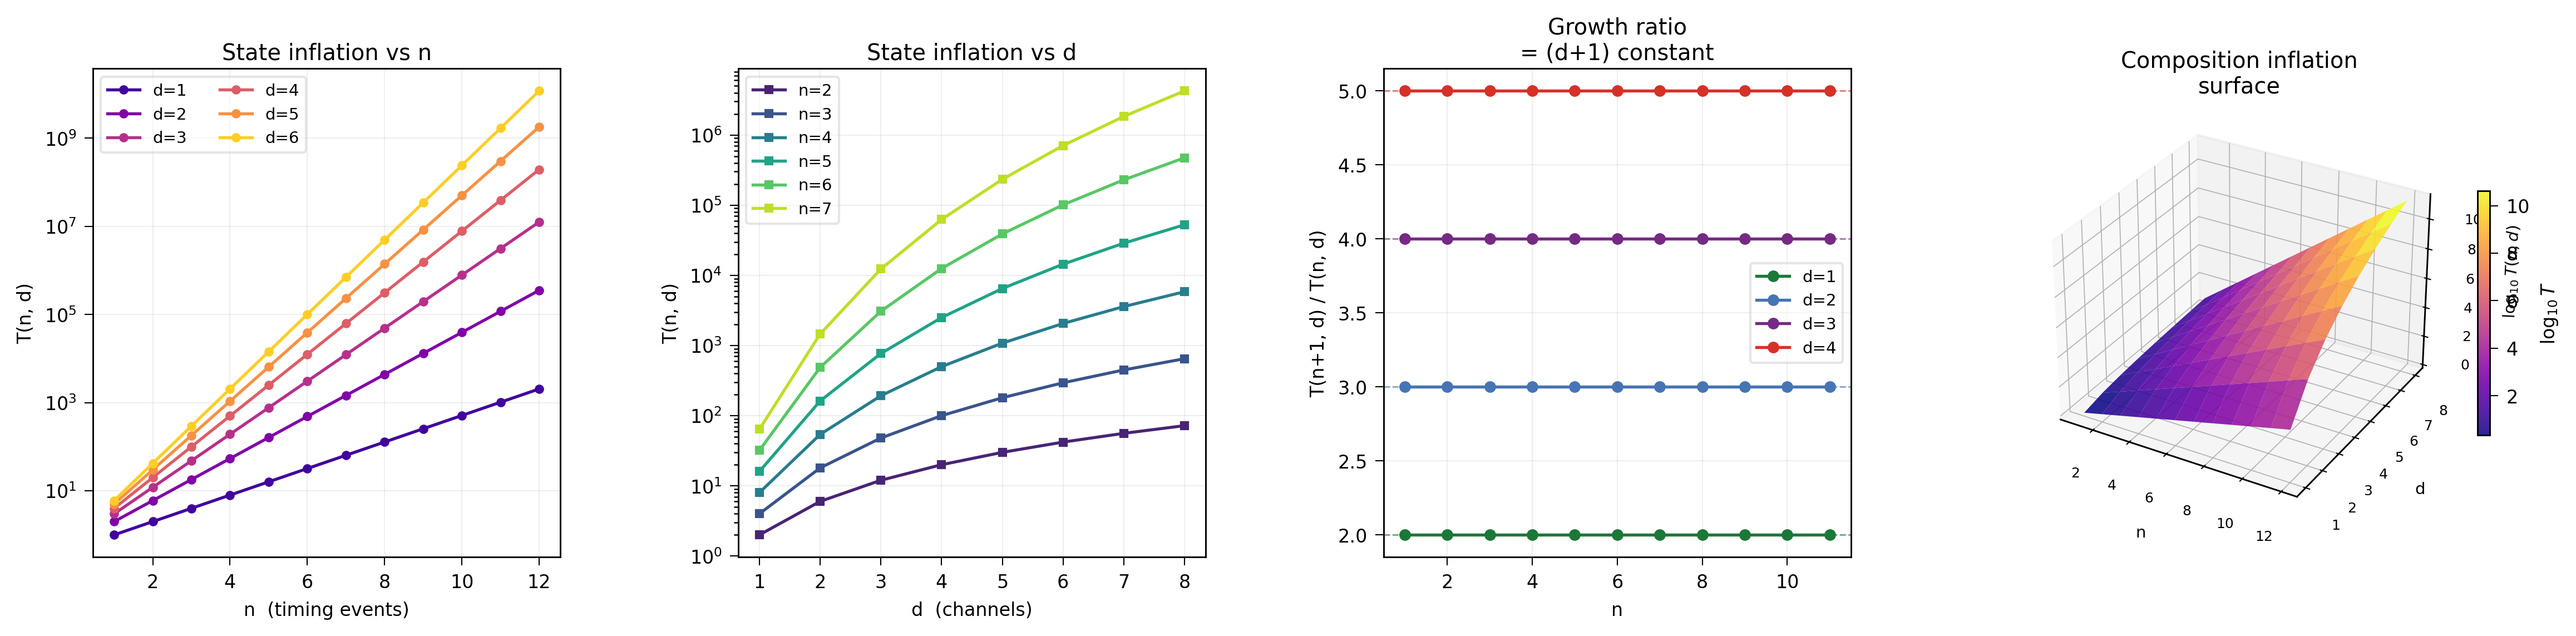
\includegraphics[width=\textwidth]{figures/panel_05_composition_inflation.png}
    \caption{\textbf{Composition-inflation $T(n,d)=d(d+1)^{n-1}$: multi-channel timing acquisition resolves an exponentially growing state space.}
    (\textbf{A}) State count $T(n,d)$ versus number of timing events $n$ on a logarithmic axis for channel counts $d=1,\ldots,6$. Each curve is a straight line in semi-log, confirming exponential growth in $n$ with base $(d+1)$; adding channels steepens the slope.
    (\textbf{B}) State count $T(n,d)$ versus channel count $d$ for event counts $n=2,\ldots,7$. The number of distinguishable states rises sharply with each additional timing channel, demonstrating the advantage of ion-mobility or multi-analyzer extensions over a single timing axis.
    (\textbf{C}) Growth ratio $T(n{+}1,d)/T(n,d)$ versus $n$ for $d=1,2,3,4$, with horizontal reference lines at $(d+1)$. Every ratio is constant and equal to $(d+1)$, providing a direct numerical verification of the recurrence $T(n{+}1,d)=(d+1)\,T(n,d)$.
    (\textbf{D}) Three-dimensional surface of $\log_{10}T(n,d)$ over the $(n,d)$ grid. The surface rises steeply in both directions, with the steepest gradient along increasing $n$ at high $d$, visualising how a two-channel IMS--MS system ($d=2$) attains a state capacity of $2\cdot 3^{n-1}$ that resolves isobars inaccessible to single-axis timing.}
    \label{fig:in-5}
\end{figure*}
